\documentclass{mcmthesis}
\mcmsetup{CTeX = false,   % 使用 CTeX 套装时,设置为 true
        tcn = 2021705, problem = D,
        sheet = true, titleinsheet = true, keywordsinsheet = true,
        titlepage = false, abstract = true}
\usepackage{newtxtext}%\usepackage{palatino}
\usepackage{lipsum}

\begin{document}
\title{From Network to Teamwork}
\begin{abstract}

In order to evaluate the game performance of the Huskies, this paper adapts multiple indicators for the data, utilizes a Structural Equation Model and proposes multiple methods.

In the fisrt part, we create a directed weighed passing network as well as a passing matrix to analyze the team's structure. At the macroscale level, we adapt five metrics from graph theory, such as the shortest path lengh, the largest eigenvalue, and the average centroid distance to measure the passing network. At the mesoscale level, we develop a novel algorithm to identify the local patterns of the network. We also create a passing matrix to recognize the diadic and triadic configurations of the team. At the microscale level, we utilize pagerank, closeness and betweeness centrality to measure the structural characteritics of a player in the network. Furthermore, we consider the these indicators from a dynamic perspective by updating them along different time scale as the match and season progresses. We discover some significant relaionship among our indicators and the team performance. 

In the second part, to better identify performance related to successful teamwork, we take the passing accuracy, invasion index and pezzali score into our consideration. Next, we divide all the indicators into four categories measuring the team's flexibility, connectivity, strength and spatial properties. Then, we assume these four categories to be latent variables and employ the Structural Equation Model to explore and filter the relationships between our indicators and the team performance. We find that the algebraic connectivity, clustering coefficient, and average centroid distance are of the most importance among them all.

In the third part, we conduct analysis and comparison on the players statistics and the team's strategies across the season. We point out the advantages and shortcomming of several players. We also point out two major offensive means of the Huskies. Then, we give our advice on the strategies for the next season.

Finally, we try to extend our indicators and models to other areas of teamwork and summarized the commonalities.
\begin{keywords}
Network, Team performance, Structural Eequations Model
\end{keywords}
\end{abstract}
\maketitle
\tableofcontents
\section{Introduction}
\subsection{Problem Restatement}
Problems which need interdisplinary knowledge, while getting much easier in the highly connected modern societies. How well a team operates may directly relate with how perfectly the problem is tackled with. Thus, we need to create a model that we can tell how the team performs given some features about it and its members.

Team sports is an example of teamwork that a team of different skills or technical characteristics work together towards a same goal of victory, where both static and dynamic features can be captured. Specifically we focus on soccer, a ball game between two teams, normally with 11 players for each side on court, both trying to kick the ball into the opponent's goal. Different strategies are implemented in soccer matches and most of them are realized by frequently passing the ball among teammates and eventually shotting it out. The passing network, which is thought to be novel perspective about team performance, has been proved to have multiple essential properties that highly related to team performance on football games. 

Requested by the coach of the Huskies, the passing network of the Huskies among 38 matches of last season is to be built. Meanwhile, structural indicators and properties of the network as well as their relation with team performance are to be investigated. These efforts should provide insights on how to improve the Huskies's performance. Furthermore, a generalized version of the model should be generated for general teamwork cases.

\subsection{Our Work}
This paper includes four following parts of our solution:
\begin{itemize}
  \item We built the passing networks of the Huskies and its opponents and plotted them on graphs. Base on the graphs, we calculated several indicators of the network structure, evaluated some network properties and, while comparing some of them between two teams.
  \item We construct multiple performance indicators from the game logs and figured out the relationship between sucessful teamwork and the team network. 
  \item Based on above discovery we suggest some pratical tatics for the Huskies to perform better in the future.
  \item We generalized the model to fit more general cases on teamwork, and tried to test it's validity.
\end{itemize}

\section{Assumptions \& Definitions}
\subsection{Assumptions}
In consideration of some realistic factors that may affect the model but are not able to be captured due to restriction on data sources, we make following assumptions to simplify our research and thus the result can be more credible:
\begin{itemize}
  \item A player's performance on the game is only dependent on personal capability, the coach's strategy, the opponent's strength and teamwork between he/she and his/her teammates while weather, mood, money and other factors that do not directly related with the game have no impact. So is the team's performance. 
  \item All players in the team or in the league remains healthy all along the season that team performances are not likely to be affected by injuries as the real world do.
  \item All players play for the same team during the season so the strategies may not be affected due to personnel changes.
\end{itemize}
\subsection{Definitions and Terminologies}
Variables used in this thesis are notated as follow:
\begin{table}[ht]
  \caption{Part of correlation matrix}
  \begin{center}
      \begin{tabular}{r|r}
          \toprule
            Terminologies & Definitions\\
          \midrule
          $G$ & Weighted directed graph representing passing network\\
          $A_{n}$ & Weighted adjacent matrix of the passing network with n nodes\\
          $D_{sum}, D_{std}$ & The sum and standard deviation of node degrees\\
          $\langle X\rangle$, $\langle Y\rangle$ & Coordinates of the network centroid \\
          $NC_{stre} $& Network dispersion\\
          $NC_{disp}$ & Network stretch index\\
          $Avg\_spl$ & Average shortest path length\\
          $\lambda_1$ & Largest eigenvalue of the adjacency matrix\\
           $\tilde\lambda_2$ & Algebraic connectivity\\
           $EC_{max},EC_{avg},EC_{std}$ & Maximum value, mean and dispersion of eigenvector centrality\\
           $Clu$ & Clustering coefficient\\
           $BC$ & Betweenness centrality\\
           $CC$ & Closeness centrality\\
           $PR$ & Pagerank\\
           $PA$ & Passing accuracy\\
           $Inv$ & Invasion index\\
           $Pez$ & Pezzali score \\
           $First50$&Timestamp that finish 50 passings\\
          \bottomrule
      \end{tabular}
  \end{center}
\end{table}
\subsection{Model Pipeline}
HERE SHOULD BE A PIPELINE
\section{Passing Network: A Graph Perspective}
In this section we construct a passing network for the passes between players to identitfy several topological-scale properties of a team. The network is a weighted directed graph with the team's players as nodes and passings from one player to another as edges, which are weighted by the number of passings. We will measure the network's connectivity, flexibility, robustness and spatial properties from micro, meso and macro perspectives.

\subsection{Weighted Directed Graph As Passing Network}
Using the data of passing events, we define the passing network as each player being a node and existing passings being directed edges, weighted by the number of passings happened on this pair of players with that direction. 

A weighted directed graph can be expressed as:
\begin{equation}
  G = (u, v, w)
\end{equation}
where $u$ represents nodes, $v$ represents edges and $w$ represents weights.

This graph can also be interpreted with the form of weighted adjacent matrix $A_n$:
\begin{equation}
  A_{n}=
  \begin{bmatrix}
      w_{11} & w_{12} & ... & w_{1n}\\ 
      w_{21} & w_{22} & ... & w_{2n}\\ 
      ... & ... & ... & ...\\ 
      w_{n1} & w_{n2} & ... & w_{nn}
  \end{bmatrix}
\end{equation}
where $w_{ij}$ equals to the number of passings directing from player $i$ and player $j$, and $n$ equal.

To better explain the passing networks, we plot them on the graph with the shape of court as background, in which the size of node denotes the number of all passings involved with this player, the arrow on the edge points to the destination player, and the size of edge denotes the number of passings happened on this route. Figure \ref{f1} shows the passing network of the Huskies and its opponent for the first match of the season, where the location of nodes on the map are the players' average passing position for this match.
\begin{figure}[htbp]
  \label{f1}
  \centering
  \caption{Passing network of match 1 for the Huskies(left) and the opponent(right)}
  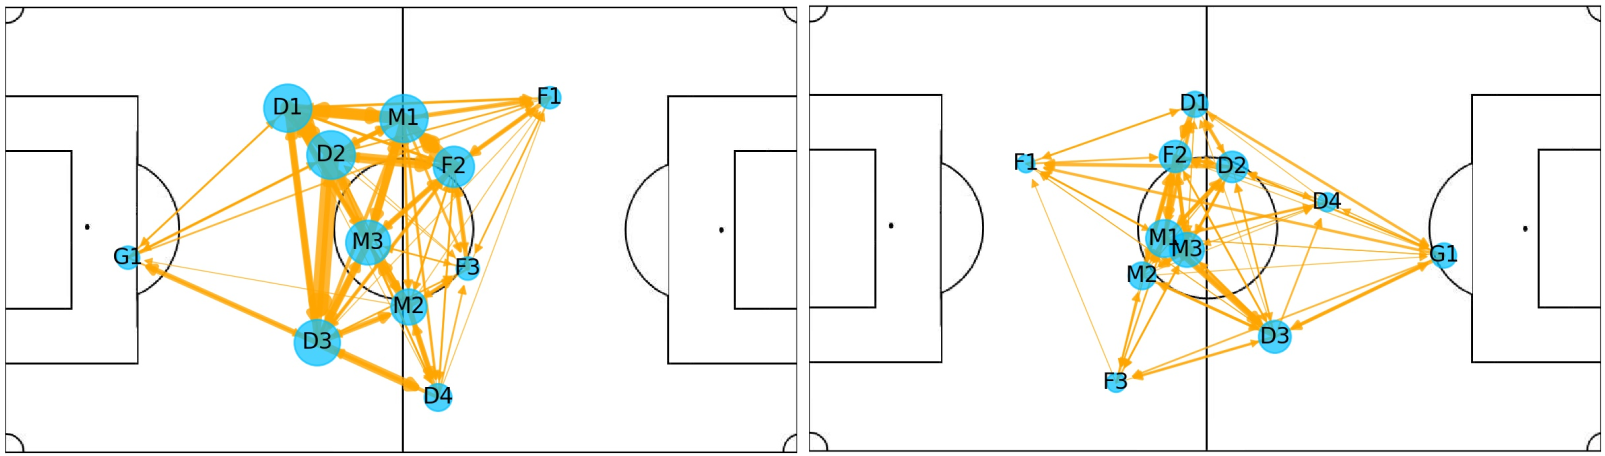
\includegraphics[width=14cm]{match1.png}
\end{figure}
To avoid players with extremely few passings affecting the general structure, we made a preprocessed the data before plotting. That is, whenever a substitution occurs, we let the new player inherit the node of the previous player. In this way, we make sure there are always exactly eleven nodes in our network.
From the passing network defined above, we measure network properties of following three scales.
\subsection{Macroscale}
At the topological macro level, we consider the network as a whole and investigate its formations. 

By fitting the nodes positions roughly correspond to the players average origin coordination on the court, we have visualized the network with a pitch map. Through categorizing the team formation for each of 38 match(Figure \ref{f1}, for example), we found that the most frequent team formations that Huskies adopted were 4-4-2 and 4-2-3-1. In most cases, the center of the team is at the center-back of the field. However, under some circumstances, i.e. when facing a strong team, the centor of the team would retreat a little in order to enhance their defense. See Figure \ref{f2}.
\begin{figure}[htbp]
  \centering
  \caption{Passing network of the Huskies versus a stronger team(left, match 5) and the normal one(right, match 34)}
  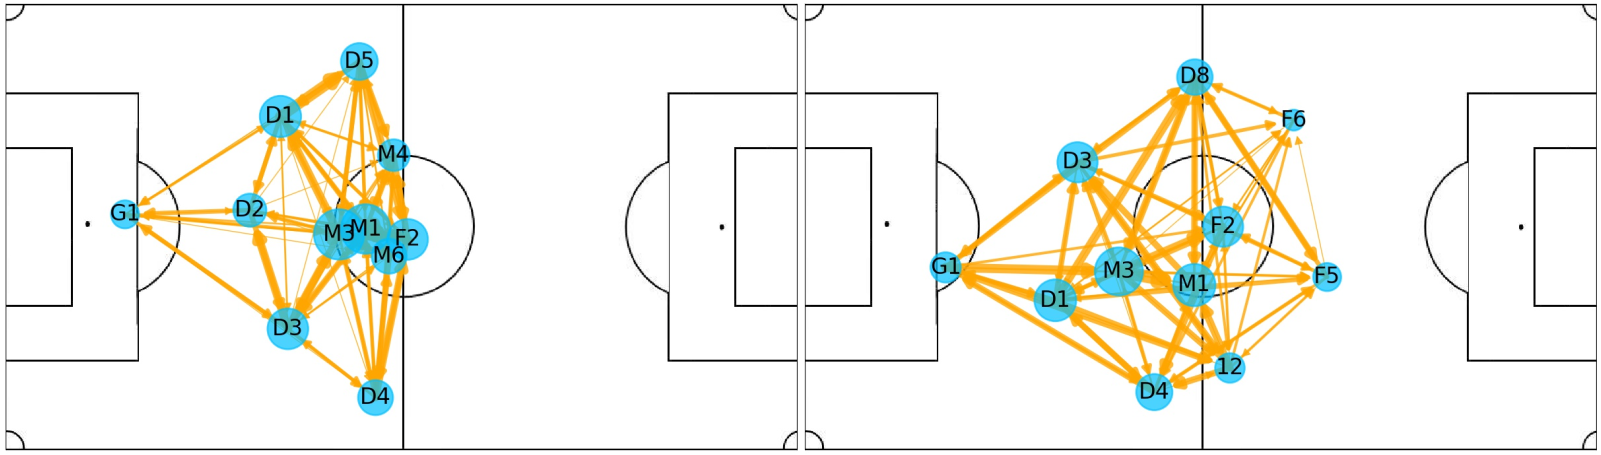
\includegraphics[width=14cm]{match2.png}
  \label{f2}
\end{figure}

On the other hand, we also construct several indicators that are informative about the network's spatial stucture, including the total number of passes and its standard deviation, coordinates of the network centroid, network dispersion and network stretch index and average shortest path length.
\begin{itemize}
  \item The sum and standard deviation of node degrees $D_{sum}, D_{std}$
  
  Node degree here represent the number of passings that the player gives and recieves. The sum of all nodes' degree represent the total number of passings in each match and while the standard deviation represent the dispersion of number of passings.
  \item Coordinates of the network centroid $\langle X\rangle,\langle Y\rangle$ 
  
  The network centroid is defined as average position of all passes of a team. To be specific, we only consider the original position of those passes, originated from the data provided. Then $\langle X\rangle,\langle Y\rangle$ are the coordinates of $x$ axis and $y$ axis, respectively. Note that for the Huskies and the opponents, the position are defined on the same coordinate system.\cite{1}
  \item Network dispersion $N_{disp}$ and network stretch index $N_{stre}$
  
  Network dispersion is defined as the standard deviation of the distances between all passings and the network centroid, and stretch idnex is the mean distance of players around the centroid. Similarly, we only consider the original positions of passes and use it as the players' coordinates as well.\cite{1}
  \item Average shortest path length $Avg\_spl$ 
  
  Average shortest path length is defined as the average length of all shortest path in the passing network between each pair of players. Note that the length $l_{ij}$ here is weighted by the inverse of link weight $l_{ij}=\frac{1}{w_{ij}}$. The shortest pathes between every two players are computed by Dijkstra’s algorithm.\cite{1} Thus, the average shortest path of the network can be denoted as:
  \begin{equation}
    Avg\_spl = \frac{1}{N(N-1)}\sum_{i,j_{i\not=j}}p_{ij}
  \end{equation}
  \item Largest eigenvalue of the adjacency matrix $\lambda_1$
  
  The largest eigenvalue $\lambda_1$ of the weighted adjacency matrix $A_n$ of a network is a measure of the network strength. A higher $\lambda_1$ usually means a higher number of links in the network and further, a more stronger aggregation of important nodes that makes the network more assortative. Which is an important matrics of network structure.\cite{1}
  \item Algebraic connectivity $\tilde\lambda_2$
  
  The algebraic connectivity $\tilde\lambda_2$ corresponds to the second smallest eigenvalue of the Laplacian matrix $\tilde{L}$, which is defined as $\tilde{L} = S - A_n$, with $A_n$ being the weighted adjacency matrix and $S$ the diagonal matrix whose $i^th$-elements are the sum of the passes made by player $i$. The algebraic connectivity is closely related to both structural and dynamical properties of networks. On the one hand, algebraic connectivity indicates the modular structure of a network: lower $\tilde\lambda_2$ means clearer existence of independent groups inside the network.\cite{1}

  \item Maximum value, mean and dispersion of eigenvector centrality $EC_{max}, EC_{avg}, EC_{std}$
  
  The eigenvector centrality $EC_i$ of a player $i$ is a measure of node importance that is obtained by calculating the eigenvector $v_1$ associated to the largest eigenvalue $λ_1$ of the weighted adjacency matrix $A_n$. Taking the number of all directed connections a node has into account, the eigenvector centrality measures node importance. Eigenvector centrality will be affected by the number of directed edges linking to the node and also importantly, the centrality of nodes where the links come from.\cite{1}

\end{itemize}

Figure \ref{macro} shows the comparision between the Huskies and the opponents on the eight properties above, where the height of the bars indicates the mean value of that property. Note that for the Huskies, the value is averaged with itself among the 38 games but for the opponents we averaged all 19 of them together.
\begin{figure}[htbp]
  \centering
  \caption{Comparision between the Huskies and Opponents on macroscale properties}
  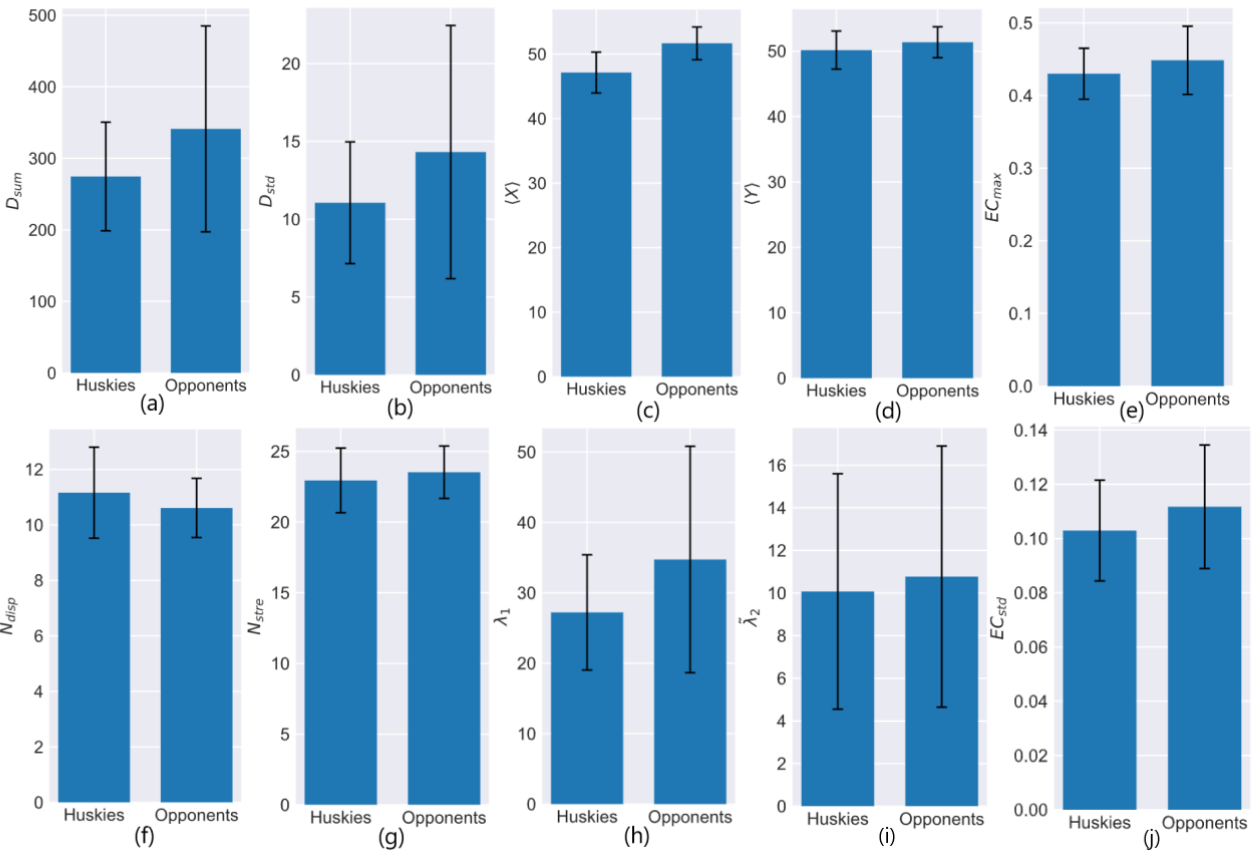
\includegraphics[width=15cm]{macro.png}
  \label{macro}
\end{figure}

We can see that on most of the macro properties, the Huskies presents a lower average value than its opponents. The only exception is the network dispersion, though the different is not really significant.

\subsection{Mesoscale}

To take a closer look at the passing network we created, we fisrt focus on certain clusters of the network to identify its mofits.  Our network is created just from the ball passing between players, but other event records in the match log such as shot, foul and ball-out event  are also userful. In this part, we split the passing events into several segments by shot, foul, and ball possession turnover events. The passing events before and after these events are considered to be in disjoint segments. In each segment, a team holds the possession of the ball. 

We developed a novel algorithm for network subgraph pattern recognithon and applied it to every disjoint passing segments. Specifically, we denote $P$ as the set of segments, into wich the match log is splited. In each segment $p_i$, for the $i_{th}$ successive passes, let $n_i$ denote the number of nodes the ball has been passed to. If $i$ is greater than $n_i$, i.e. the edges outnumbres the nodes in a subgraph, we assume the process of such passing of ball to be a teamwork. The corresponding motif of the subgraph is considered to be a network tactic pattern.

After counting the number of times that various tactic patterns have appeared, we extracted the most frequent and representative pattern and marked the players involved.See Figure\ref{meso}.

We analyze the learned tactical patterns as well as coordinates of the players and the players' role in tactical layout. For example, Figure \ref{meso}(b) can be viewed as a defensive pattern, with repeatedly passes between different defenders and midfielders, while Figure \ref{meso}(c) shows attack in two wings and figure1 indicates a kind of outflanking pattern.
\begin{figure}[htbp]
  \centering
  \caption{Multiple player tatic patterns of the Huskies}
  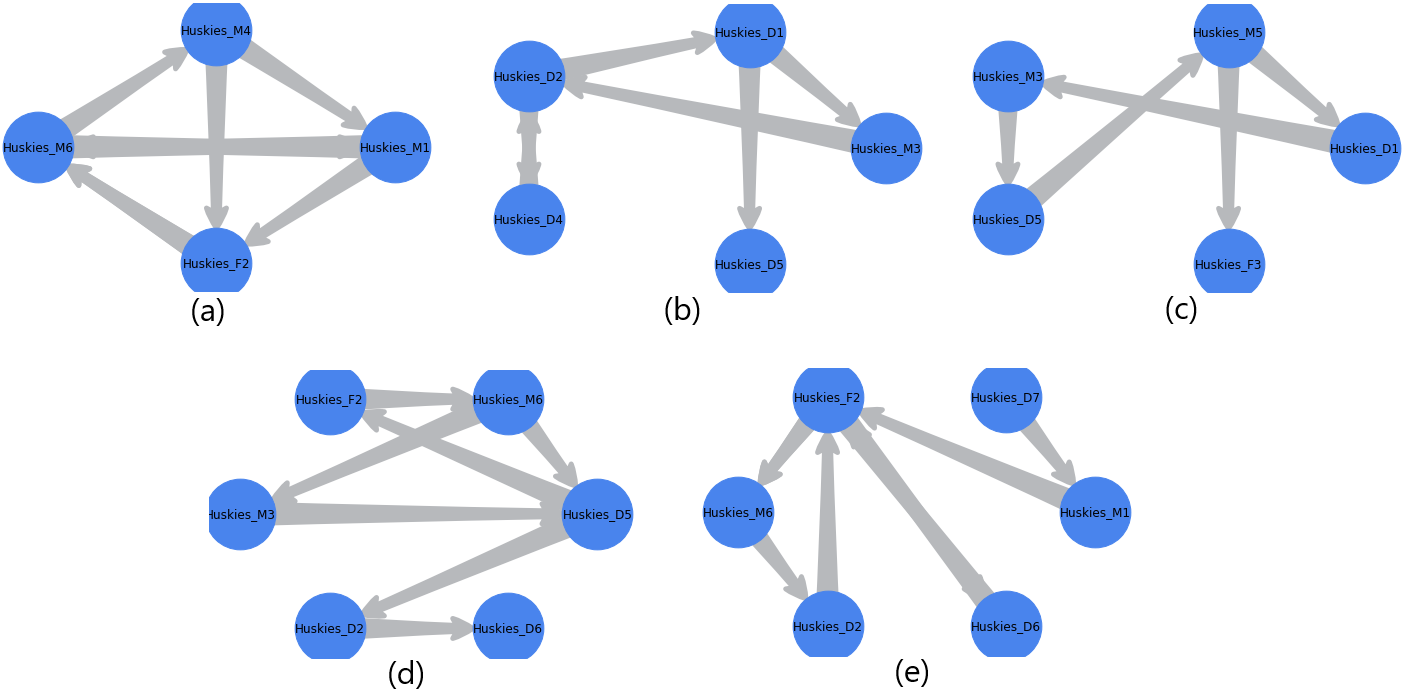
\includegraphics[width=15cm]{meso1.png}
  \label{meso}
\end{figure}
\subsubsection{Dyadic configuration}

For the dyadic configuration, we built a passing matrix from our passing network to help analyze the passes between players. To better identify the passing feature between pairwise players, we extracted the passes made by the players before each shot events, since we assume the dyadic teamwork for passing mainly occurs while the team is attacking. (When the team is defending, passes are usually made by the opponent, who takes the possession of the ball.)Therefore, we also added the shot events into our matrix.
\begin{figure}[htbp]
  \centering
  \caption{Dyadic configuration of the Huskies}
  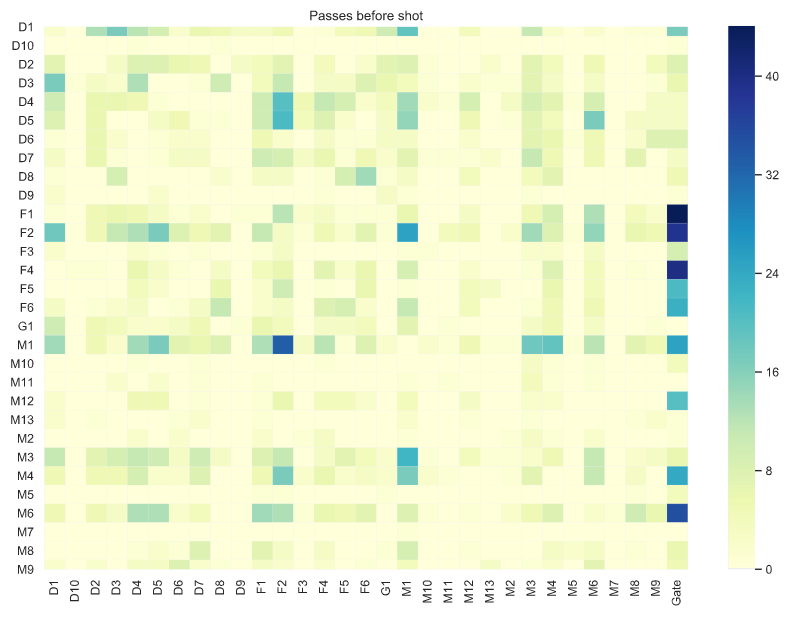
\includegraphics[width=10cm]{dyadic.png}
  \label{dyadic}
\end{figure}
The pass matrix is displayed in the form of a heat map Figure \ref{dyadic}, in which the darker the block, the more passes were made by the two players. The last column, with the x coordinate, Gate, represent the total number of shots by the player. 

From Figure \ref{dyadic} we can see that passes between Huskies F2, the core player of the team, and other players such as D1, D5 and M6 were very frequent. Also, there were a number of pasees between M1 and M4, M1 and M5, indicating the close coperation between them. Moreover, Figure \ref{dyadic} also shows that F1, F2, F4, M6 have the top 4 shots in the season. In detail, among these four players, F4 contributed a lot of shot, but not many passed, while the other three player had many shots as well as passes.

\subsubsection{Triadic configuration}

With respect to the triadic configurations, the clustering coefficient can be used to measure the triangulation between three nodes (i.e. players).

For weighted graphs, the clustering coefficient is defined as the geometric average of the subgraph edge weights,
\begin{equation}
  Clu_u = \frac{1}{deg(u)(deg(u)-1))} \sum_{uv} (\hat{w}_{uv} \hat{w}_{uw} \hat{w}_{vw})^{\frac{1}{3}}
\end{equation}

The edge weights $\hat{w}_{uv}$ are normalized by the maximum weight in the
network $\hat{w}_{uv} = \frac{w_{uv}}{\max(w)}$.The value of $Clu_u$ is assigned to 0 if $\deg(u)<2$.

In practical, for a triangle connecting three players exists, whenever a link (i.e. pass) between two players is lost (for example, obstructed by an opponent), there is still an alternative way of reaching the other node passing through the other two edges of the triangle. In general, this is an indicator of the local robustness of the network.\cite{2}

\subsection{Microscale}

At the microscale level, we use the following indicators to identify the players role and its importance inside the network.

\begin{itemize}
  \item Betweenness centrality: $BC$
  
  We use betweeness centrality to measure how the ball-flow between other players depends on a particular player.
  
  The betweenness centrality of a node $v$ is defined as the sum of the fraction of all-pairs shortest paths that pass through $v$.
  \begin{equation}
    BC(v) =\sum_{s,t \in V} \frac{\sigma(s, t|v)}{\sigma(s, t)}
  \end{equation}

  where $V$ is the set of nodes, $\sigma(s,t)$ is the number of shortest $(s,t)$-paths, and $\sigma(s,t|v)$ is the number of those paths passing through some node $v$ other than s,t. If $s=t$, $\sigma(s,t)=1$, and if $v\in s,t$,$\sigma(s,t|v)=0$.
  
  Also, this indicator helps us analyze the impact of removing that player from the game, either by getting a red card or by being isolated by the rival's defense. A betweenness score of 0 means, in particular, that a player is not getting involved in the game.
  \item Closeness centrality: $CC$
  
  Considering the accesibility of a player in the passing network, we want to know whether a players is easy to reach when other plays choose to pass. Therefore, we introduce the closeness centrality.
  
  The closeness centrality of a node $u$ is the reciprocal of the average shortest path distance to $u$ over all $n-1$ reachable nodes.
  \begin{equation}
    CC(u)=\frac{n−1}{\sum^{n−1}_{v=1}d(v,u)}
  \end{equation}

  where $d(v, u)$ is the shortest-path distance between v and u, and n is the number of nodes that can reach $u$. 

  It's worth to point out that the "distance" defined in this indicator is not a spatial distance, but a tactical distance, measured by the reciprocal of the number of passes between players. A player with low closeness may indicate that this player cannot reach the ideal position to catch the ball or that he is heavily surrounded by defenders. On the contrary, a high closeness score corresponds to a small average distance, indicating a well-connected player within the team.\cite{2}

  \item Pagerank: $PR$
  
  Pagerank is designed to indicate the importance of a node in a network. It was first proposed by Google and applied to the ranking of the importance and popularity of web pages. Similarily, this indicator can be applied to our passing network to measure a player's popularity.\cite{3}

  The pagerank centrality is defined by
  \begin{equation}
    PR_i = p\sum_{j\not=i}\frac{A_{ji}}{L^{out}_j}PR_j + q
  \end{equation}
\end{itemize}

where $L^{out}_j = \sum_kA_{jk}$ is the total number of passes made by player $j$, $p$ is a heuristic parameter representing the probability that a player will decide to give the ball away rather than keep it and go for a shot himself, and $q$ is a parameter awarding a 'free' popularity to each player. Intuitively, a player is popular if he gets passes from other popular players.

Note that the pagerank of a player depends on the pagerank of all his teammates.

\subsection{Temporal evolution for network properties}

As we have seen in previous subsection, all the indicators are construct and calculated based on the seasonal scale average. Specifically, we inspected the changes of indicators match by match and further update them to cover the rolling window containing every 50 passes in each match. 

\subsubsection{Match-to-match Scale}
In order to preliminary study the relationship between the above indicators and the performance of the game, select indicators that can be further analyzed. First of all, we use the difference between the index of the Huskies and the opponent team in each game as the ordinate, and draw a line chart of the directly observable variables and the winning and losing relationship. The following figure is an example of six indicators, which are $D_{sum}$ (the sum of the number of passes), $D_{std}$ (the standard deviation of the number of passes), clustering coefficient $Clu$, $\lambda_1$(largest eigenvalue of the adjacency matrix), $\tilde\lambda_2$(algebraic connectivity), average shortest path length $Avg\_spl$:
\begin{figure}[htbp]
  \centering
  \caption{Network properties of the Huskies match by match}
  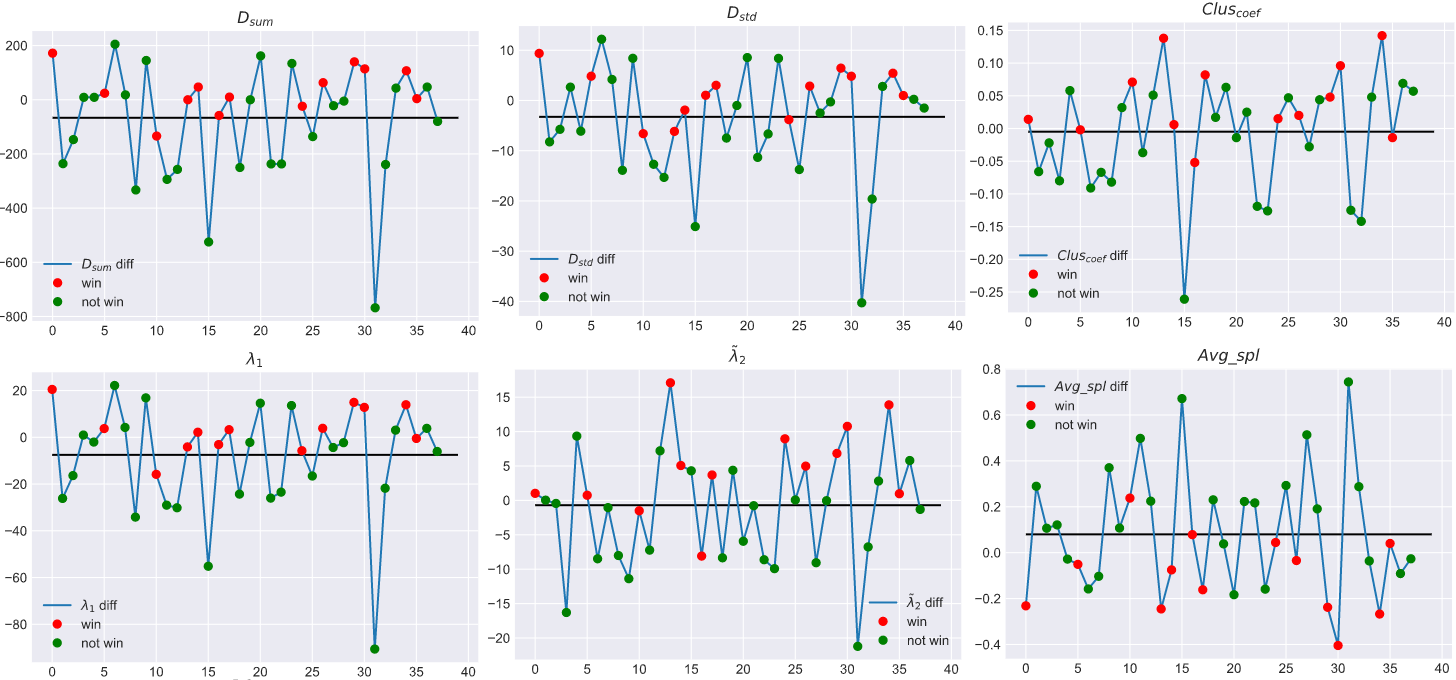
\includegraphics[width=15cm]{mtom.png}
  \label{match}
\end{figure}


\subsubsection{50 Passes Rolling Window}

Since the situation on the court is always changing rapidly, the performance of the teams may diverse a lot during a game. Therefore, from a dynamic perspective, it's necessary to update our indicators inside match progresses. \cite{1}
\begin{figure}[htbp]
  \centering
  \caption{Network properties of the Huskies in 50 passes rolling window}
  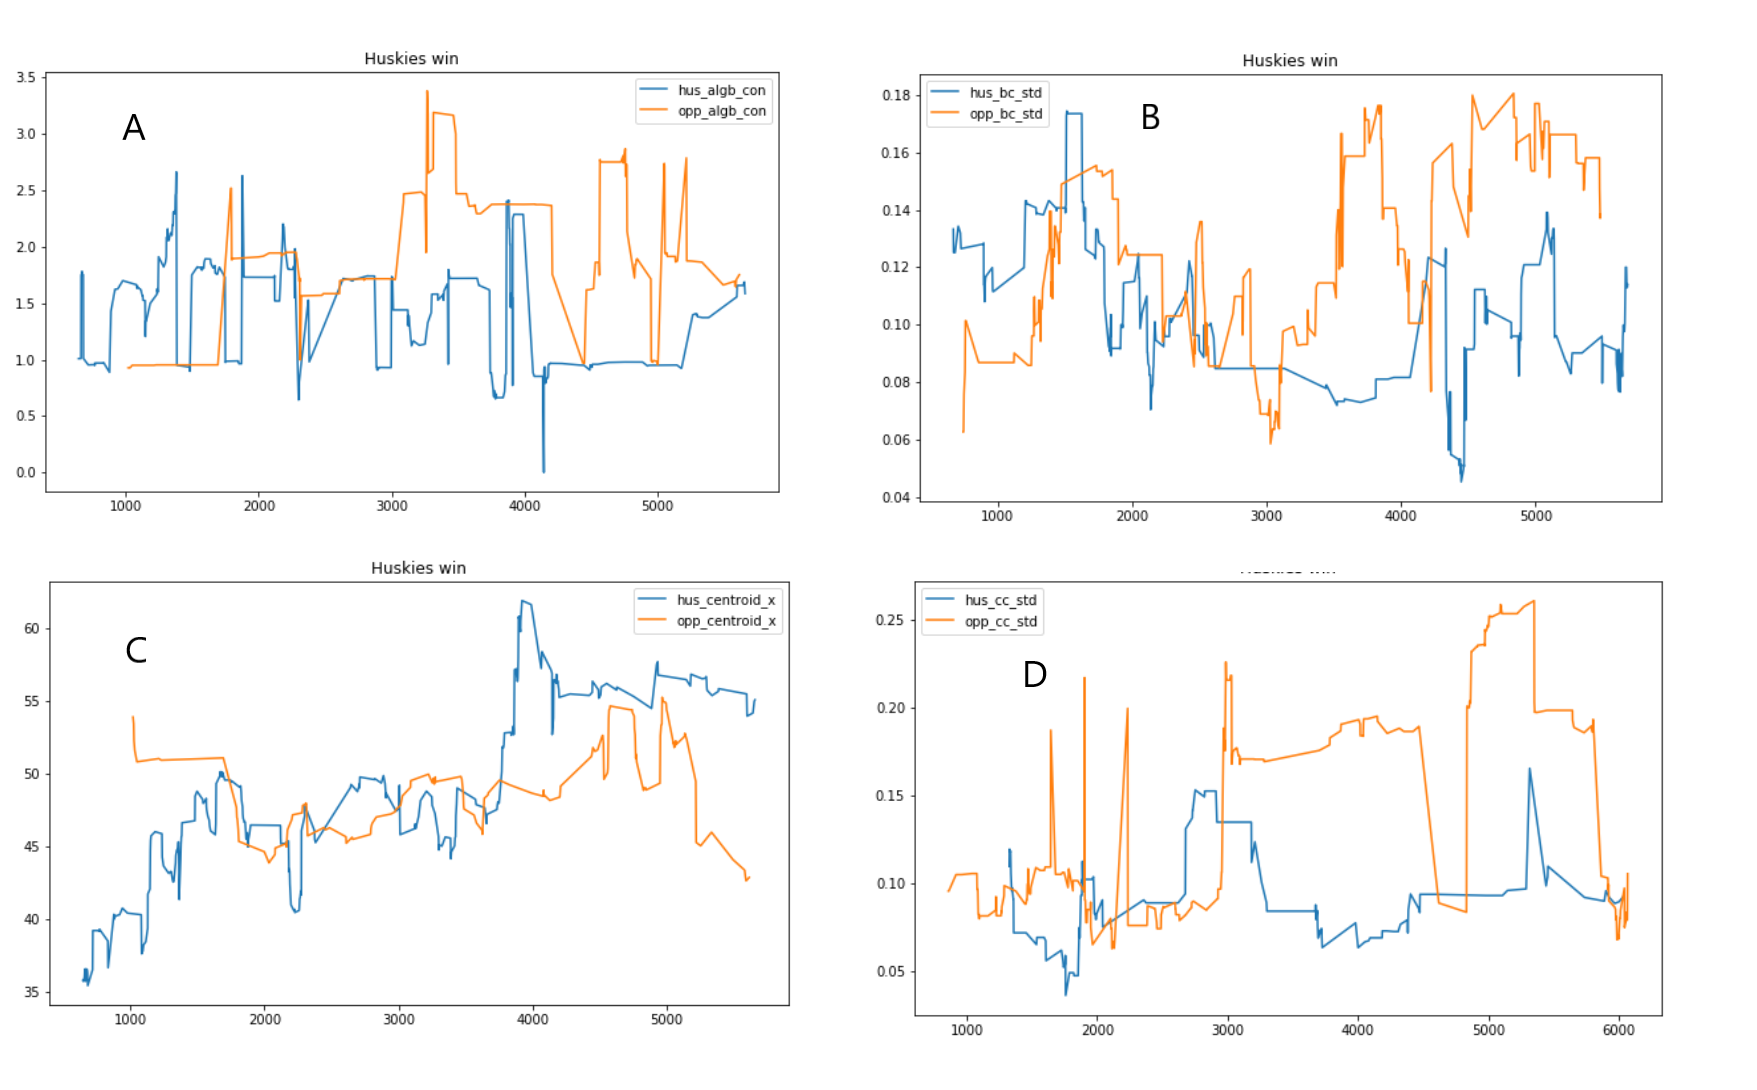
\includegraphics[width=15cm]{temporal.png}
  \label{temporal}
\end{figure}

Figure \ref{temporal} shows an example of a time window diagram of four indicators of two teams in a match according to every 50 passes. Specifically, (A)algebraic connectivity $\tilde\lambda_2$, (B)betweenness centrality $BC$ , (C)x-coordinate of centroid$\langle X\rangle$, (D)closeness centrality$CC$.

Figure \ref{temporal}(A) Shows whether the team's passing network has obvious sub-networks, that is, the existence of independent mutual passing tactics. It can be clearly seen that in the entire game, this indicator of the Huskies is less volatile than the opponent, indicating that the Huskies is more even and scattered in the application of tactics, which represents a style of the Huskies' game mode.

Figure \ref{temporal}(B) is the standard deviation of betweenness centrality. According to the previous introduction, betweenness measures the participation of each node to some extent. The lower the standard deviation, the more even the responsibility sharing of the entire team is. It can be shown that the participation of all players in the second half of the game is more average than the first half, and the player participation is higher.

Figure \ref{temporal}(C) shows the team moving to the front and back positions during the game. In the game shown by C, you can see that the Huskies gradually changed from defensive to offensive posture in the second half. This may be the result of a change in game style or tactical changes.

Figure \ref{temporal}(D) We can observe that the centrality standard deviation of the opponent team rises sharply after 50 minutes. The centrality standard deviation shows the importance of players. The sharp rise may be because the opponent team has adopted some tactics to make the ball holding rate of some people suddenly high, or because the Huskies defense makes it difficult for some opponents to get the ball.



\section{Measuring Team Performance: Indicators and Structural Equation Model}

\subsection{Performance indicators}

In addition to the most direct outcome, such as scores that the team made, goal difference between the team and its opponent and whether the team wins or not, we construct some other indicators that can also reveal team performance. Details are listed below:
\begin{itemize}
  \item Passing accuracy: $PA$
  
  In terms of the performance indicators that reflect successful teamwork, we natually use the passing accuracy indicator. To do so, we first counted the passes between teammates (successful passes) and the number of passing event that caused an turnover of the possession of the ball (passing failure). The passing accuracy is calcudated by
\begin{equation}
  PA = \frac{successful \  passes}{successful \  passes + passing \  failures}
\end{equation}
\begin{figure}[htbp]
  \centering
  \caption{Passing accuracy of the Huskies' Players}
  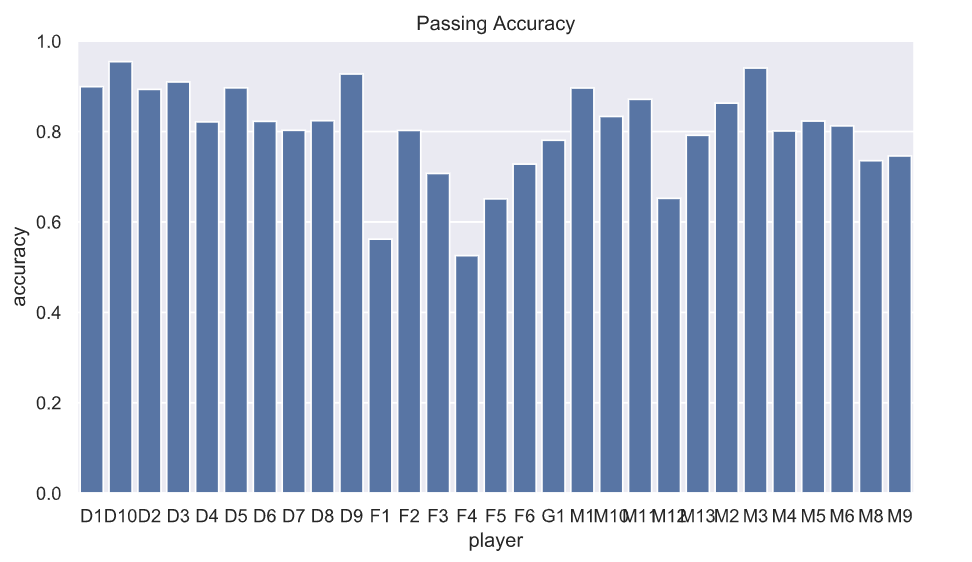
\includegraphics[width=12cm]{pa.png}
  \label{pa}
\end{figure}

Figure \ref{pa} shows the average passing accuracy of each player in the season.

  \item Invasion index: $Inv$
  
  In order to measure the effectiveness of a team's offensive tatics, we take the invasion index into consideration.
  
  The invasion index is calculated through the following steps:
  First, split the match events into disjoint segments according to the team's continuous possession of the ball. Then for each event in the segment, its scoring probability is defined as the fraction of goals that have been scored from that position where the event take place.
\begin{equation}
  scoring \  probability= \frac{1}{1+e^{\frac{distance}{k}-1}}
\end{equation}

After that, for each segment, take the highest of all events' scoring probabilities as the segment's scoring probability. 
A team' s overall invasion index during a match is simply the average invasion index across its segments. Note that since we do not have the record about when and where the goals were achieved, we use the record of shots instead. See Figure \ref{inv}.\cite{1}

\begin{figure}[htbp]
  \centering
  \caption{Scoring probabilities distribution of the Huskies' Players}
  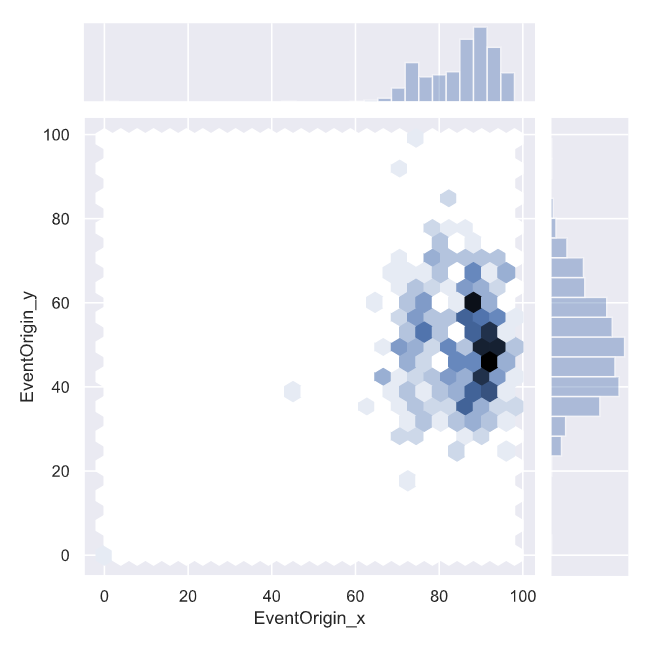
\includegraphics[width=8cm]{inv.png}
  \label{inv}
\end{figure}

Figure \ref{inv} show the distribution of the scoring(shoting) probability on the field. Dark area means that there have been many shot event occured in it, which leads to a high probability of shot.

  \item Pezzali score: $Pez$
  
  Another indicator of team efficiency is the pezzali score, which considers the efficiency for both attack and defense. Accoring to Pezzali, football matches follow "the harsh rule of goal: you play a great game but if you don't have a good defense, the opponent scores and then wins". \cite{5}

  For each team and each game we obtain a defense/attack efficiency rate, then the pezzali score is calculated with:
  \begin{equation}
    Pez = \frac{attempts(team)}{possession(team)}\times\frac{possession{opponent}}{attempts(opponent)}
  \end{equation}

  High Pezzali score of a team indicates that the team is highly effective both in attack and defense, i.e. it needs few attempts to score a goal (low ratio goals/attempts) and the opponent needs many attempts to score a goal (high ratio goals/attempts). Conversely, the Pezzali score of a team is low when the team is ineffective both in attack and defense: it needs many attempts to score a goal while the opponent needs few attempts to score a goal.

  \item Timestamp that finish 50 passings: $First50$
  
  From rolling windows, we can also obtain a indicator: denoted as $First50$ and defined as the time that a team complete 50 passes in a match.\cite{1} It measure the frequency of passing in the initial part of the math and indicates how fast the team get into a "competition mode".
\end{itemize}



\subsection{Model Construct: Structural Equation Model(SEM)}

From a network propestive, we construct a structural equation model to capture different aspects of teamwork including structural, configurational and dynamic properties. 

Structural equation model is a statistical method to analyze the relationship between variables based on the covariance matrix of variables. It is a combination of confirmatory factor analysis and latent variable causal model. The part of the factor model is the measurement model, and the equations in it are the measurement equations, which describe the relationship between the latent variable and the watchable indicator.

The general version of structural model can be expressed as following three eqations:
\begin{equation*}
  \begin{split}
    x &= \Lambda_x \xi + \sigma \\
    y &= \Lambda_y \eta + \epsilon \\
    \eta &= B\eta + \Gamma\xi + \zeta
  \end{split}
\end{equation*}
where $x$,$y$ are obtainable indicators vectors, $\xi$,$\eta$ are latent variables, $\Lambda_x$,$\Lambda_y$,$B$,$\Gamma$ denote the relationship between $x$ and $\xi$, $y$ and $\eta$, $\eta$ and $\eta$, $\eta$ and $\xi$, respectively.

The exploration steps are generally divided into the measurement of latent variables, the analysis of exploratory factors, and the analysis of confirmatory factors.

By observe into correlation between so much varibales defined above, we notice some variables with relatively high correlation as the following table:

\begin{table}[ht]
  \caption{Part of correlation matrix}
  \begin{center}
      \begin{tabular}{r|rrrr}
          \toprule
            & $net\_win$&$PA$&$Pez$&$First50$\\
          \midrule
           $\tilde\lambda_2$ & 0.32 & 0.18 & -0.08 & -0.18\\
           $\lambda_1$ & 0.33& 0.76 & 0.46 & -0.56\\
           $Clu$ & 0.21 & 0.34 & 0.05& -0.31 \\
           $Avg\_spl$ & -0.37 & -0.69 & -0.18 & 0.68\\
           $BC_{avg}$ & -0.33 & -0.61 & -0.18 & 0.60\\
           $CC_{avg}$ & 0.30 & 0.44 & 0.11 & -0.41\\
           $EC_{avg}$ & 0.16 & -0.15 & -0.21 & 0.10\\
           $PR_{max}$ & 0.05 & 0.01 & 0.05 & 0.13\\
           $NC_{stre}$ & 0.09 & 0.10 & 0.00 & 0.03\\
           $\langle X\rangle$ & 0.16 & 0.27 & 0.05 & -0.17\\
          \bottomrule
      \end{tabular}
  \end{center}
\end{table}

Restrict by space we can only exhibit limited part of the correlation matrix but we can see that some of them are highly correlated that relations might hide behind them.

According to the previous analysis, we decided to perform an structural analysis into the relationship between network and teamwork, thus we build a structural equations model which is well suited with our problem setting that some variables cannot be directed measured. And performance indicators first include all of the network properties mentioned before. Through exploration, the latent variables and their measurement variables are defined based on four categories: 
\begin{itemize}
  \item Network connectivity $Conn$: Algebraic connectivity $\tilde\lambda_2$, Largest eigenvalue of the adjacency matrix $\lambda_1$, Clustering coefficient $Clu$.
  \item Network flexibility $Flex$: Average shortest path length $Avg\_spl$, Mean of Betweenness Centrality$BC_{avg}$, Mean of Closeness Centrality $CC_{avg}$.
  \item Network Strength $Stren$: Mean of Eigenvalue Centrality $EC_{avg}$, Maximun of Pagerank $PR_{max}$
  \item Spatial properties of network $Spat$: Network stretch index $NC_{stre}$, x-coordinate of network centroid $\langle X\rangle$
\end{itemize}
Besides, we selected several other indicators that are not directly relative to the network as complementary explanation variables to team performance $Perf$: goal difference of each game, pass accuracy, time that complete 50 passes in a match.
Observed variables (indicators of team performance) are: goal difference $net\_win$, pass accuracy $PA$, pezzali score $Pez$, time to complete the first 50 passes $First50$.

Then we construct measurement models as follows:
\begin{equation}
  \begin{split}
    Conn &=\sim \tilde\lambda_2 + \lambda_1 + Clu \\
    Flex  &=\sim Avg\_spl + BC_{avg} + CC_{avg} \\
    Stren &=\sim EC_{avg} + PR_{max} \\
    Spat &=\sim NC_{stre} + \langle X\rangle \\
    Perf &=\sim net\_win + PA + Pez + First50 \\
  \end{split}
\end{equation}

And the regression model is like this:

\begin{equation}
  Perf \sim Conn + Flex + Stren + Spat
\end{equation}

\begin{figure}[htbp]
  \centering
  \caption{Structural Equation Model for Teamwork Performance}
  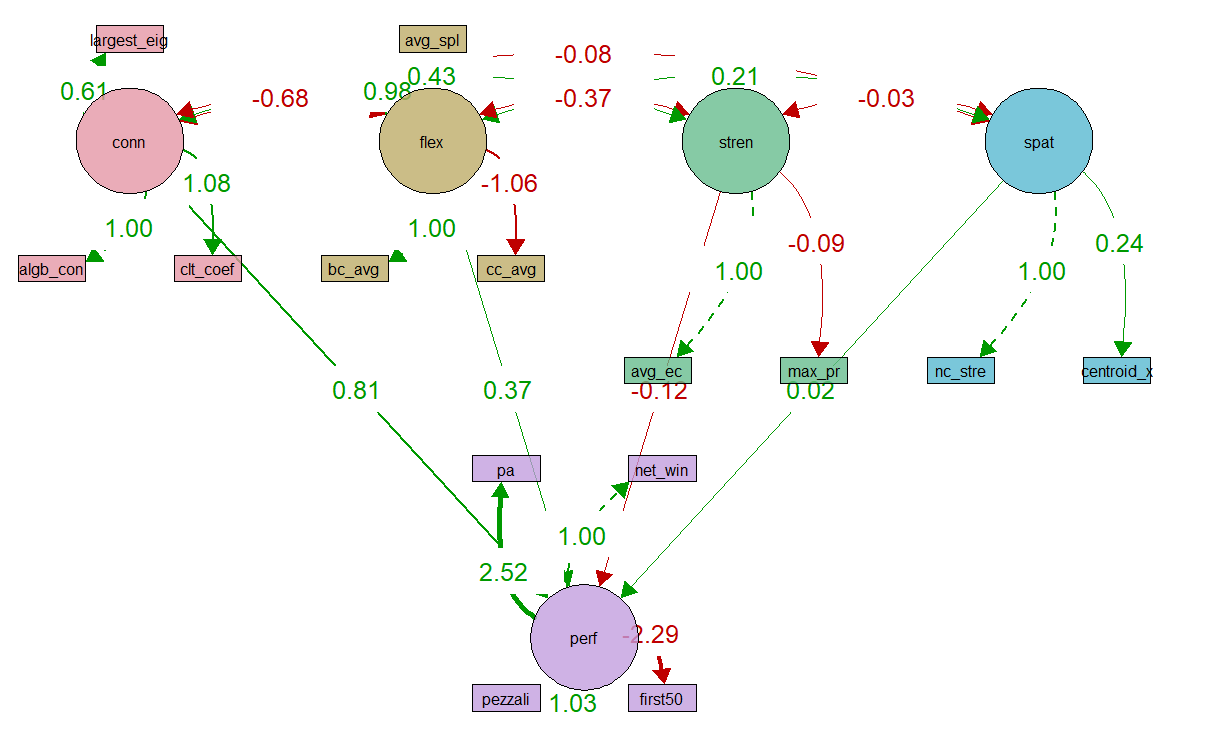
\includegraphics[width=15cm]{sem.png}
  \label{sem}
\end{figure}
After observation and fitting, we obtained the final structual model with coefficients reported as in Figure \ref{sem} and can be interpreted as below:
\begin{equation}
  \begin{split}
    Conn &= \tilde\lambda_2 + 0.61\lambda_1 + 1.08Clu \\
    Flex  &= Avg\_spl + 0.43BC_{avg} - 1.06CC_{avg} \\
    Stren &= EC_{avg} -0.09 PR_{max} \\
    Spat &= NC_{stre} 0.24 \langle X\rangle \\
    Perf &= net\_win + 2.52PA + 1.03Pez - 2.29First50 \\
    Perf &= 0.81Conn + 0.37Flex + -0.12Stren + 0.02Spat
  \end{split}
\end{equation}

\section{Strategies Making}
\subsection{Seasonal Review}
\subsubsection{player analysis}

Based on our data, the performance of a player's personal ability can be evaluated by his passing accuracy, number of shots per match, number of duals per match, as well as his pagerank in the network of the team.
\begin{figure}[htbp]
  \centering
  \caption{Player Analysis over season}
  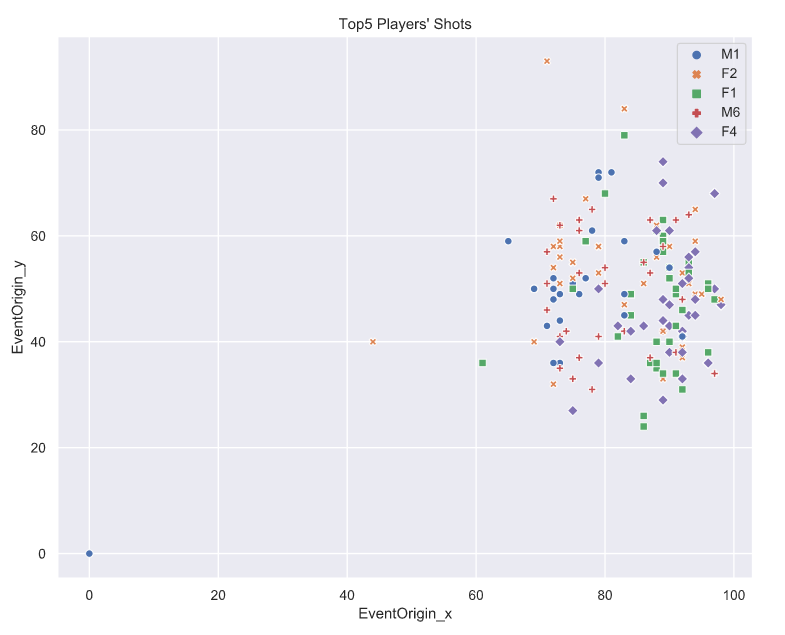
\includegraphics[width=10cm]{player.png}
  \label{player}
\end{figure}

Figure \ref{player} shows the postion where the shots were made by the top players of the Huskies. For player F4, we can see that his shooting area is mainly in fron of the gate, probably because of his excellent body and ability to perform header shots. With respect to F2, he usually launch shots from the outside of the penalty area.

In terms of the other indicators, for the reason that players in difference position on the team are likely to have different statistics on average, we will consider and compare players' performance indicators accoding to their tactic position.

Specificly, we divide player in to three catgories: front, center, and defender (denoted as F, M, D respectively) and plot the value of their performance indicator over matches in the season. In addition, since some players only played just a few games throughout the season, for each positon, we only show the top 3 players who played the most games. See Figure \ref{12p}.
\begin{figure}[htbp]
  \centering
  \caption{Player Analysis over season}
  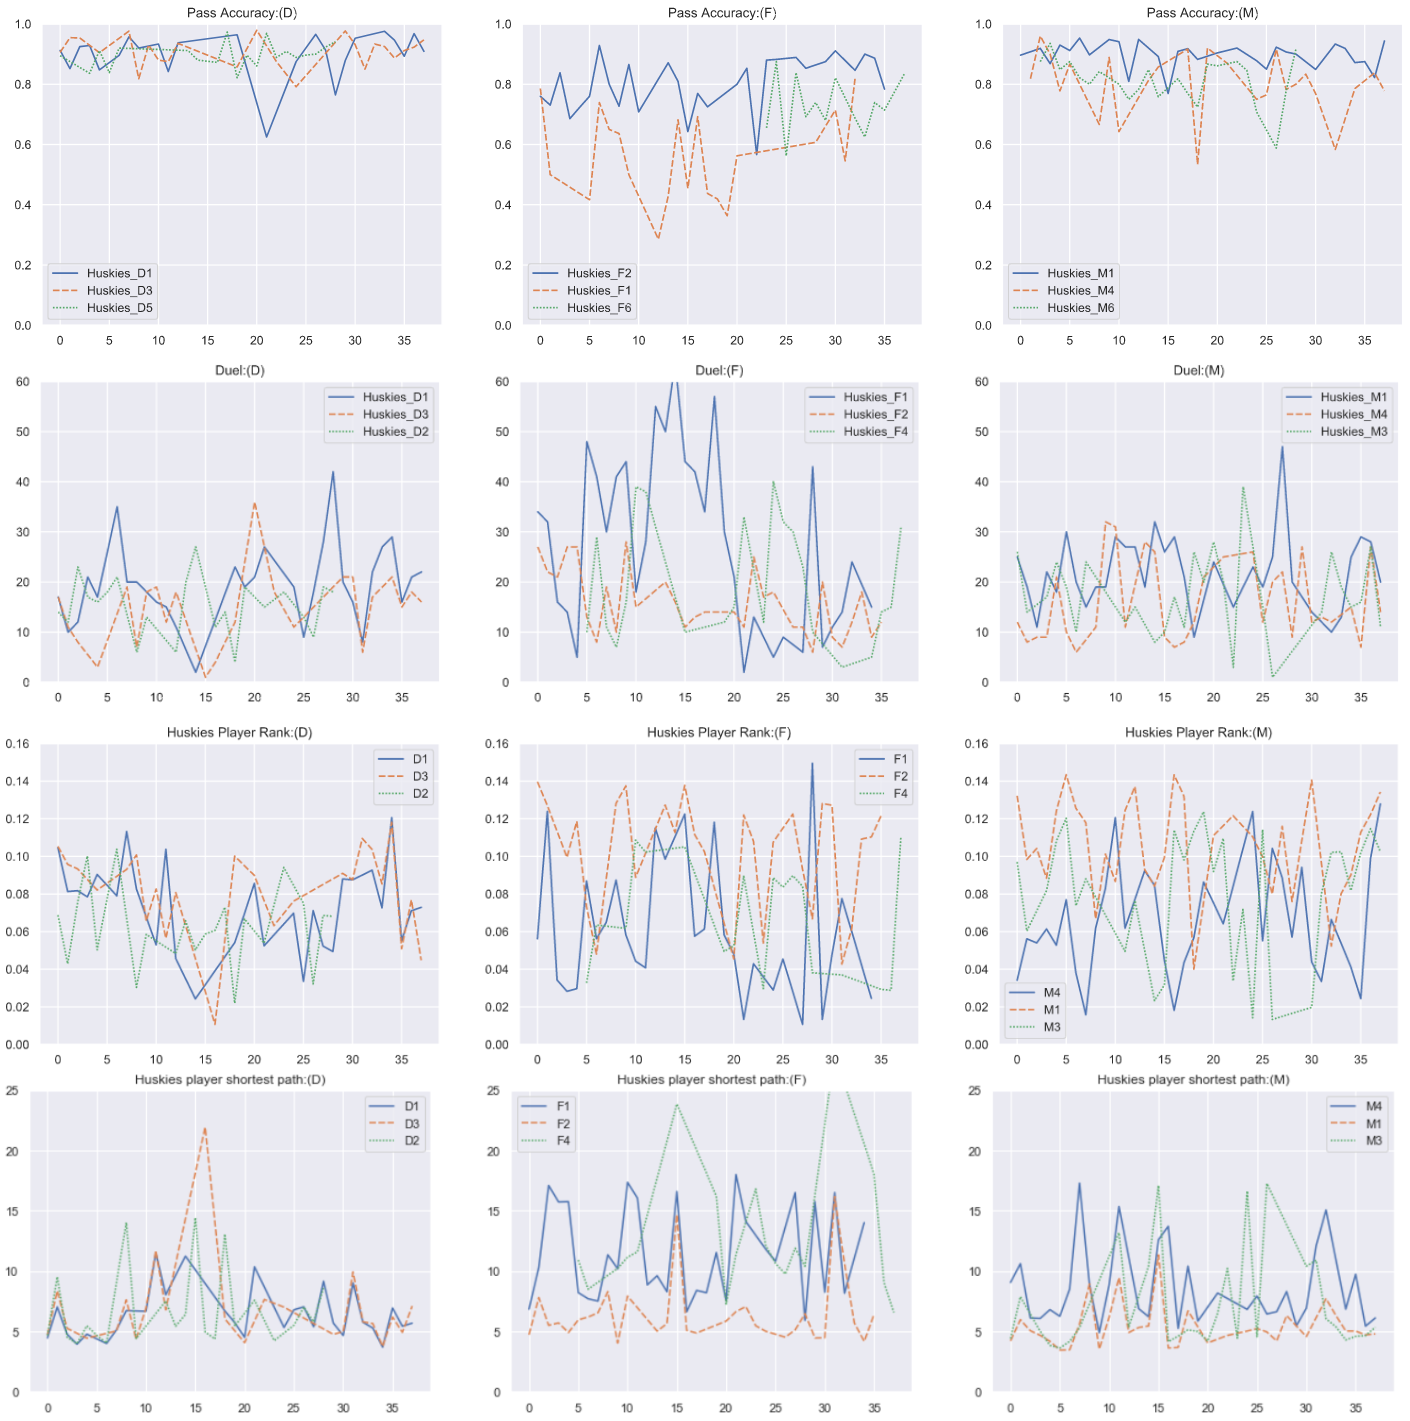
\includegraphics[width=15cm]{12pics.png}
  \label{12p}
\end{figure}

Taking the the forwad position as an example( the middle column in figure 7): player Huskies F2 significantly outperforms the reset of the players. In addition to his high passing accuracy and player rank, Huskies F2's average shortest path is clearly low than others, which indicates his extrodinary ability of choosing the shortest path when making a pass. Also, it's worth noting that  the total number of duels of Huskies F1 is very high, which may mean that he's been very active on the field, espetially in the first few games.

\subsection{Team Analysis}
To excavate and recognize tactics that have been successful for the Huskies, we set the "shot event" as the signal of a successfull tactic and use a "event window" to pickout the last 10 event records before the shot. Based on these event records, we visualize the successive passes before the shot as well as the the oppnent players' positions on the pitch. (Bule nodes represent Huskies players and red nodes are opponent players. The nodes' positions are the coordinates of the destination of a event. See Figure \ref{shot}.) 
\begin{figure}[htbp]
  \centering
  \caption{Player Analysis over season}
  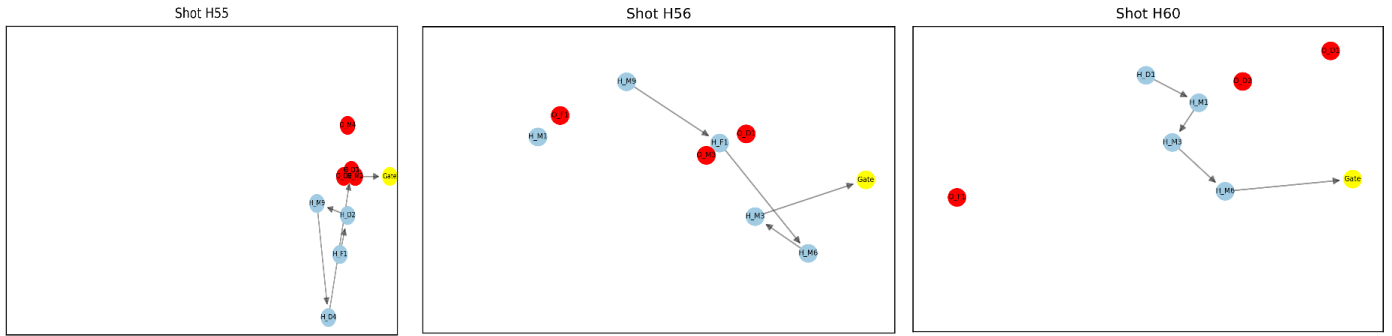
\includegraphics[width=15cm]{shot.png}
  \label{shot}
\end{figure}
Through our analysis, we find that a great deal of attacks share the same pattern. The Huskies often find oppotunities to attack on the oppenent's ribs. To be specific, the center players of the Huskies have a great ability to cut in from the sides of the field and pass the ball to the middle, where the front players can lauch a shot. 

\begin{figure}[htbp]
  \centering
  \caption{Player Analysis over season}
  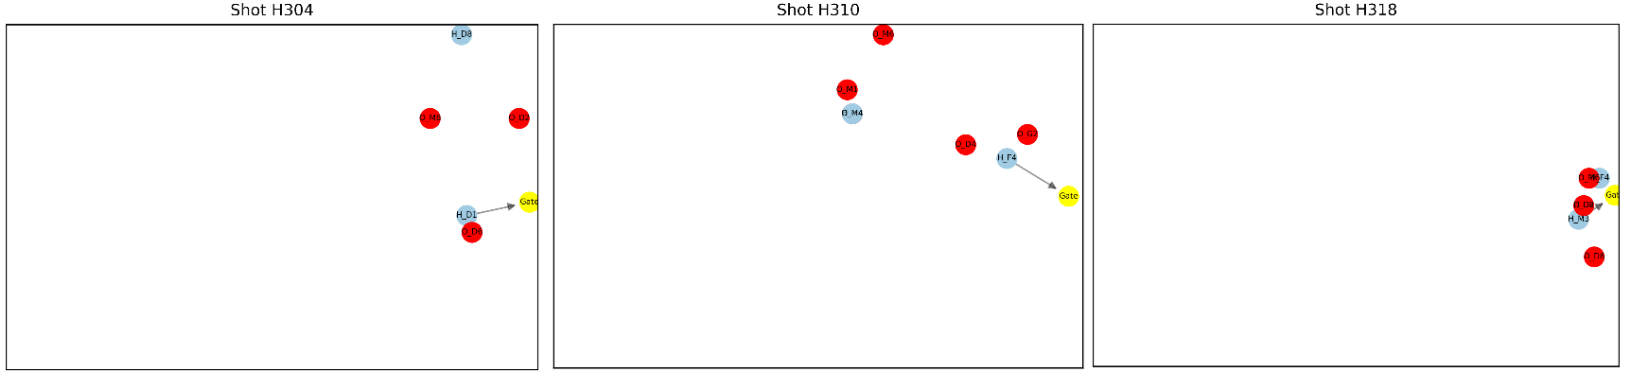
\includegraphics[width=15cm]{shot2.png}
  \label{shot2}
\end{figure}

In addition, thanks to the outstanding personal ability of the forward players (M3, F4, F1), "steal and shot"(Figure \ref{shot2}) in the frontcourt is also an important effective offensive means.

\subsection{Advice For Next Season}

In terms of the offensive means, we suggest the Huskies to develop more offensive means next season, such as crossing from the botton line. Correspondingly, the front players should improve their ability of header shot.

From the perspective of network indicators, we suggest the coach of the Huskies to seek betweenness centrality scores that are evenly distributed among players, because concentrated betweenness scores indicate a high dependence on few, too important players, whereas well distributed, low betweenness scores are an indication of a well-balanced passing strategy. What's more, at the mesoscale level, we advise the players to try to maintain the network pattern of triangles and try to enhance the strength of the edges. Finally, our observation of the invasion index of the Huskies and its opponents indicates that there is some gap between the attack efficiency of the Huskies and that of it opponents, espetially in thoses lost games. Practically, to improve the Huskies attack efficiency, we suggest the players to start attacking more decisively when they get the ball, rather than making conservative passes.

\section{More Than Football}

From the perspective of team dynamics, the team atmosphere consists of several aspects:
\begin{itemize}
  \item Group pressure and group standards
  \item Leadership and group performance
  \item Group structure
\end{itemize}

In the model constructed in the previous analysis, we quantified the influence of various indicators of the team on the performance of the team: The centroid coordinate measures the situation of attack or defense, and corresponds to the pressure value facing the group. The player's pagerank reflects the leadership abilities of some players, and the standard deviation of the ball's holding time reflects the distribution of players' responsibility and average pay; The clustering of the network shows the existence of small groups in the team. The maximum envalue quantifies the team's robustness. Connectivity and flexibility, mapping to the team can be seen as the efficiency of communication between members, etc. These indicators together quantify the team's structure.

In this analysis, through the mapping of specific indicators to various aspects of group dynamics, we can roughly conclude that an efficient team needs a certain degree of external pressure; Small groups with close ties are needed, but individual members who are too important can have an adverse effect on efficiency; Teams need a group structure with high robustness, flexibility, and connectivity to enable all parties to communicate quickly and effectively.

In addition to the data that has been provided, for football, you also need the ability value data of each player, the player's career record, the time of the goal, the coaching team data, etc .For broader team analysis, time data of members "effectiveness in the team, measurement of team members" capabilities, etc. are required.

\begin{thebibliography}{99}
\bibitem{1} Guardiola's F.C. Barcelona, J. M. Buldú, J. Busquets, I. Echegoyen\& F. Seirul.lo. Defning a historic football team: Using Network Science to analyze. 19 September 2019.
\bibitem{2} Javier M. Buldú, Javier Busquets,  Johann H. Martínez, José L. Herrera-Diestra, Ignacio Echegoyen, Javier Galeano7 and Jordi Luque. Using Network Science to Analyse Football Passing Networks: Dynamics, Space, Time, and the Multilayer Nature of the Game October, 2018.
\bibitem{3} Javier Lopez Pe ´ na˜ and Hugo Touchette†. A network theory analysis of football strategies. July 2, 2012.
\bibitem{4} Qing Wang, Yuan Yao. Discerning Tactical Patterns for Professional Soccer Teams: An Enhanced. August 2015.
\bibitem{5} Paolo Cintia, Luca Pappalardo, Dino Pedreschi, Fosca Giannotti, Marco Malvaldi. The harsh rule of the goals: data-driven performance indicators for football teams. October 2015
\bibitem{6} https://networkx.github.io/documentation/networkx-1.9.1/. NetworkX documentation. September 20, 2014

\end{thebibliography}

\end{document}
